\documentclass[11pt]{beamer}
\usetheme{Pittsburgh}
\usepackage[utf8]{inputenc}
\usepackage{amsmath}
\usepackage{amsfonts}
\usepackage{amssymb}
\usepackage{undertilde}
\usepackage{bm}
\usepackage{subcaption}
\usepackage[table]{colortbl}

\graphicspath{{./images/}}

%\usepackage{sansmathaccent}
%\pdfmapfile{+sansmathaccent.map}

\author[N. Miller]{Nathan Miller}
\title{Micromorphic Finite Element Method}
%\setbeamercovered{transparent} 
%\setbeamertemplate{navigation symbols}{} 
%\logo{} 
%\institute{
\includegraphics[width=1.8in]{./Boulder_one_line.pdf}} 
%\date{} 
%\subject{}

\newcommand{\TEN}[1]{\underline{\underline{#1}}}
\newcommand{\VEC}[1]{\utilde{#1}}
\newcommand\defeq{\mathrel{\stackrel{\makebox[0pt]{\mbox{\normalfont\tiny def}}}{=}}}
\newcommand{\LTN}[1]{\left|\left| #1 \right|\right|}
\newcommand{\dev}[1]{\text{dev}\left(#1\right)}

\setbeamercolor{title}{fg=black,bg=white}
\setbeamercolor{frametitle}{fg=black,bg=white}
\setbeamercolor{itemize item}{fg=black,bg=white}
\setbeamercolor{enumerate item}{fg=black,bg=white}
\setbeamercolor{local structure}{fg=black}

\setbeamertemplate{headline}[text line]{
\vspace{1pt}
\insertshortauthor\hfill\insertshorttitle\hfill\insertframenumber
}

\setbeamertemplate{footline}[text line]{

\includegraphics[width=1.0in]{Boulder_FL.pdf}\hfill
}
\setbeamertemplate{navigation symbols}{}
\addtobeamertemplate{footline}{\rule{\paperwidth}{1pt}\vspace{1pt}}{}

\setbeamertemplate{itemize items}[default]
\setbeamertemplate{enumerate items}[default]

\begin{document}

{
\setbeamertemplate{headline}{}

\begin{frame}[noframenumbering]
\titlepage
\end{frame}
}
%\begin{frame}
%\tableofcontents
%\end{frame}
\begin{frame}{Motivation}

\begin{itemize}
\item {Heterogeneous materials are common in engineering applications
\begin{itemize}
\item Concrete/asphalt/sand
\item Metals at grain scale
\item Polymer bound crystalline materials (Asphalt/Propellants/Plastic Explosives
\end{itemize}
}
\item {Modeling is quite difficult
\begin{itemize}
\item Large deformations in small regions (shear banding)
\item Stresses at the micro level have a profound impact on stresses on the continuum
\item ``The macro-scale response is \textbf{driven} by the behavior of material in the tails of the distribution of stress/strain/temperature etc.''
\end{itemize}
}
\end{itemize}

\end{frame}

\begin{frame}{Motivation}

\begin{figure}
\centering
\includegraphics[width = 0.7\textwidth]{./images/shear_banding.pdf}
\caption{“Shear bands in dense metallic granular materials,” Hu, N; Molinari J.F., J. Mech. Phys. Solids, Vol 52, No. 3, 2002}
\end{figure}

\end{frame}

\begin{frame}{Motivation}

\begin{figure}
\centering
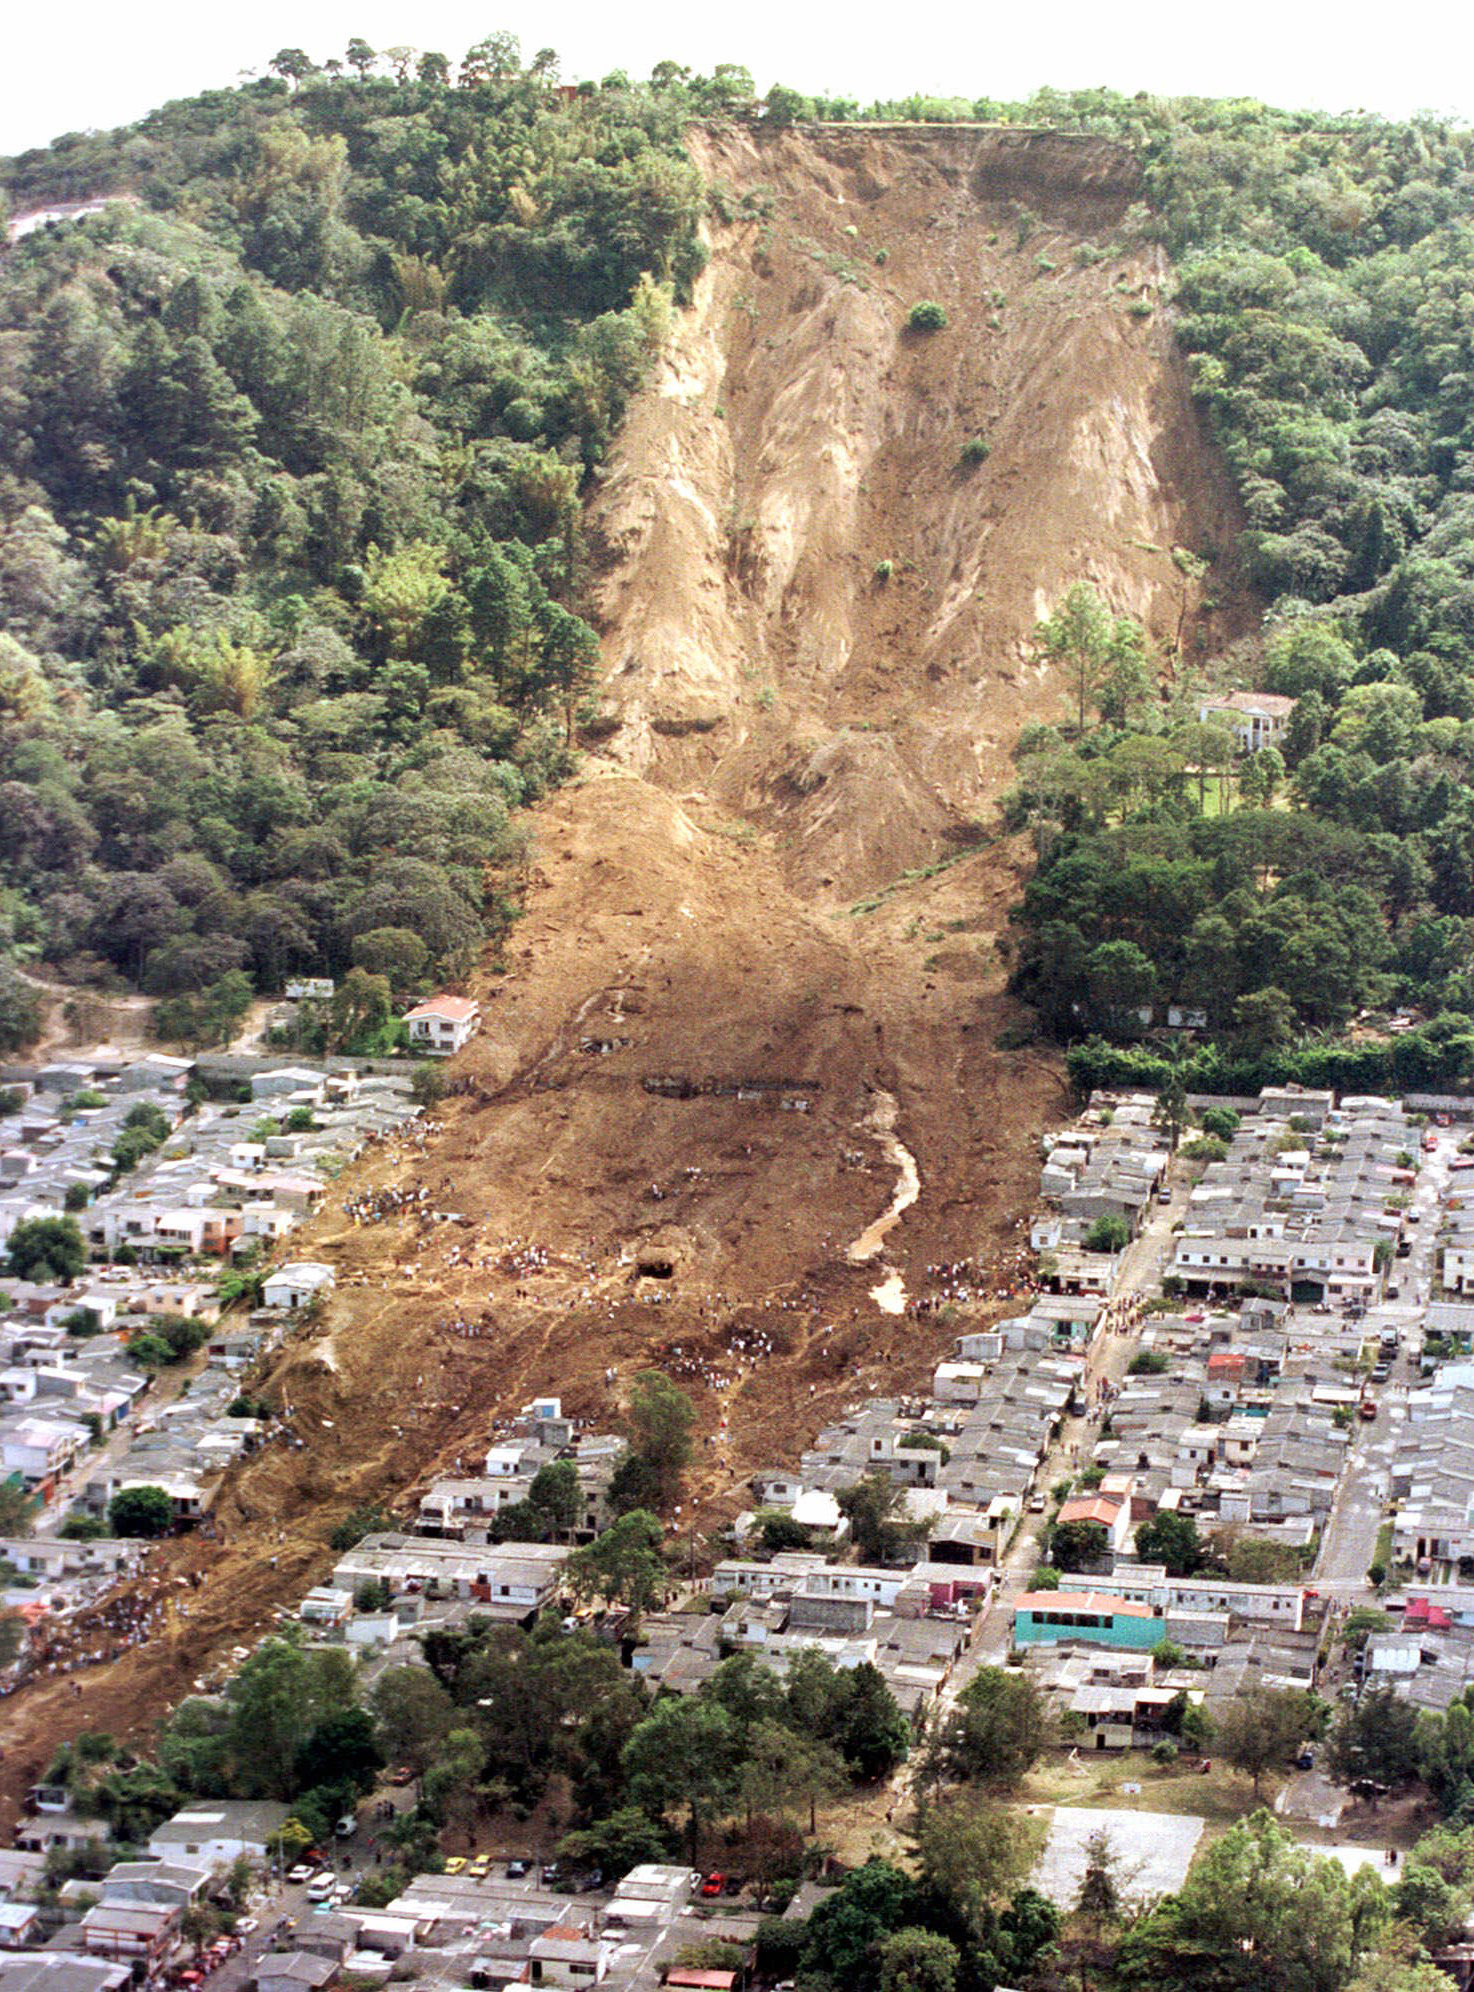
\includegraphics[width = 0.37\textwidth]{./images/landslide.jpg}
\caption{“Landslide during the 2001 El Salvador Quake” courtesy of USGS from wikipedia.org }
\end{figure}

\end{frame}

\begin{frame}{Motivation}

\begin{figure}
\centering
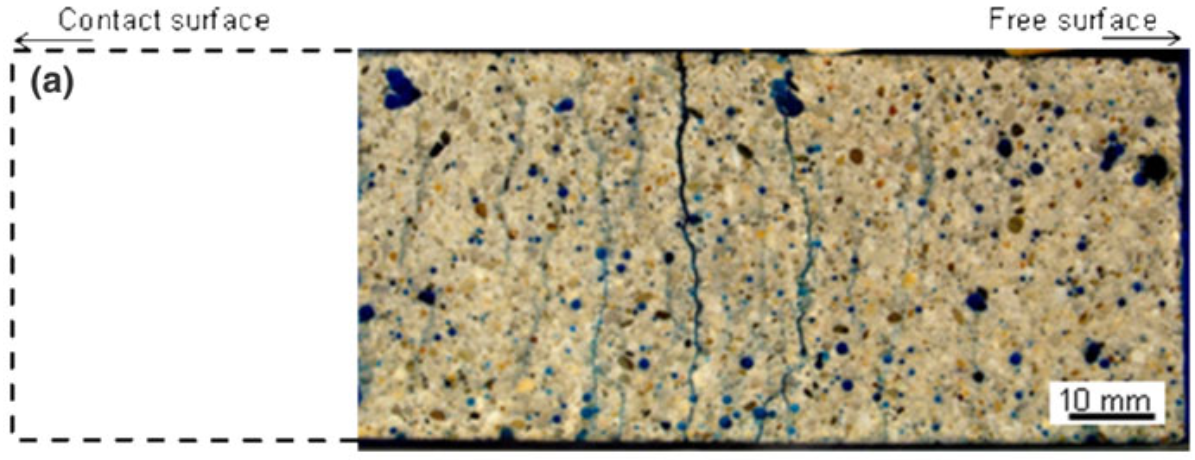
\includegraphics[width = 0.9\textwidth]{./images/impact_spalling.png}
\caption{“Dynamic fragmentation process in concrete under impact and spalling tests,” Forquin, P.; Erzar, B., Int. J. Fract, Vol. 163, pg. 193-215, 2010}
\end{figure}

\end{frame}

\begin{frame}{Motivation}

\begin{figure}
\centering
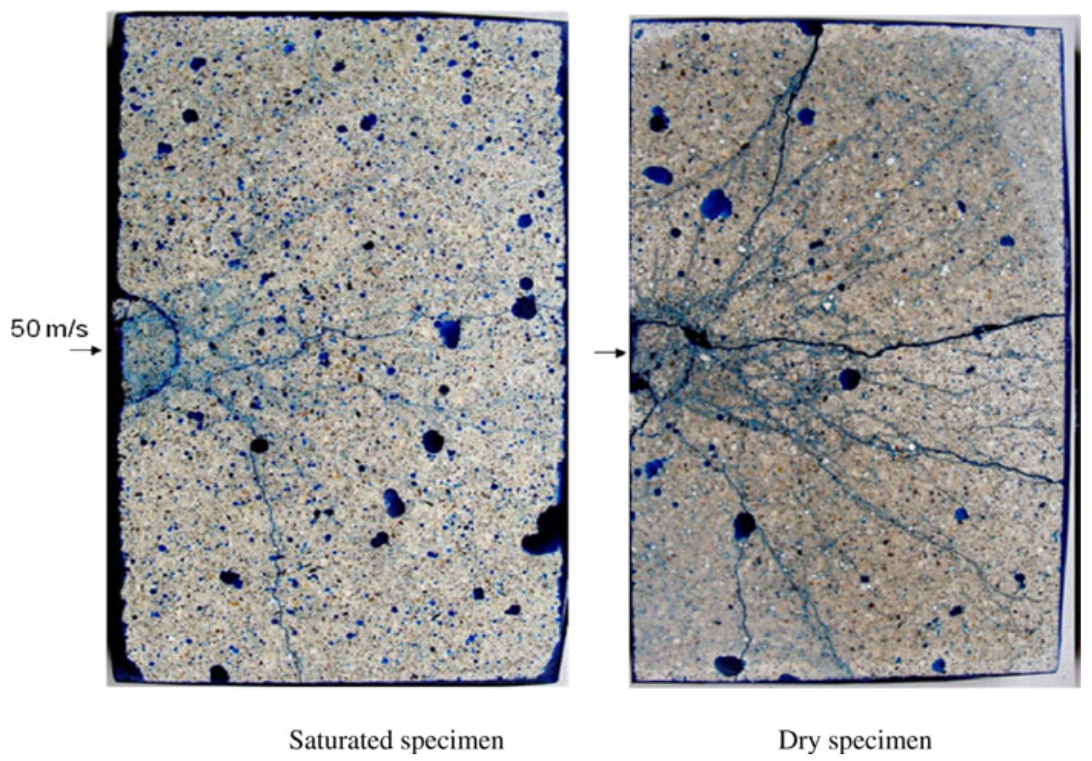
\includegraphics[width = 0.65\textwidth]{./images/impact_fracture.png}
\caption{“Dynamic fragmentation process in concrete under impact and spalling tests,” Forquin, P.; Erzar, B., Int. J. Fract, Vol. 163, pg. 193-215, 2010}
\end{figure}

\end{frame}

\begin{frame}{Motivation}
We seek a method which will allow us to incorporate the micro-displacements into the continuum level response in such a way that we maximize the amount of data available to us, minimize the amount of smearing, and allow for easy coupling between the macro and micro scales.
\end{frame}

\begin{frame}{Micromorphic Description}
Micromorphic continuum mechanics offers a solution to part of the puzzle
\begin{columns}
\begin{column}{0.5\textwidth}
\begin{itemize}
\item Extension to traditional continuum mechanics
\item A secondary vector (assumed small) from initial vector
\item Heterogeneity is a fundamental part of the approach
\item Not limited to one solution technique
\end{itemize}
\end{column}
\begin{column}{0.5\textwidth}
\begin{figure}
\centering
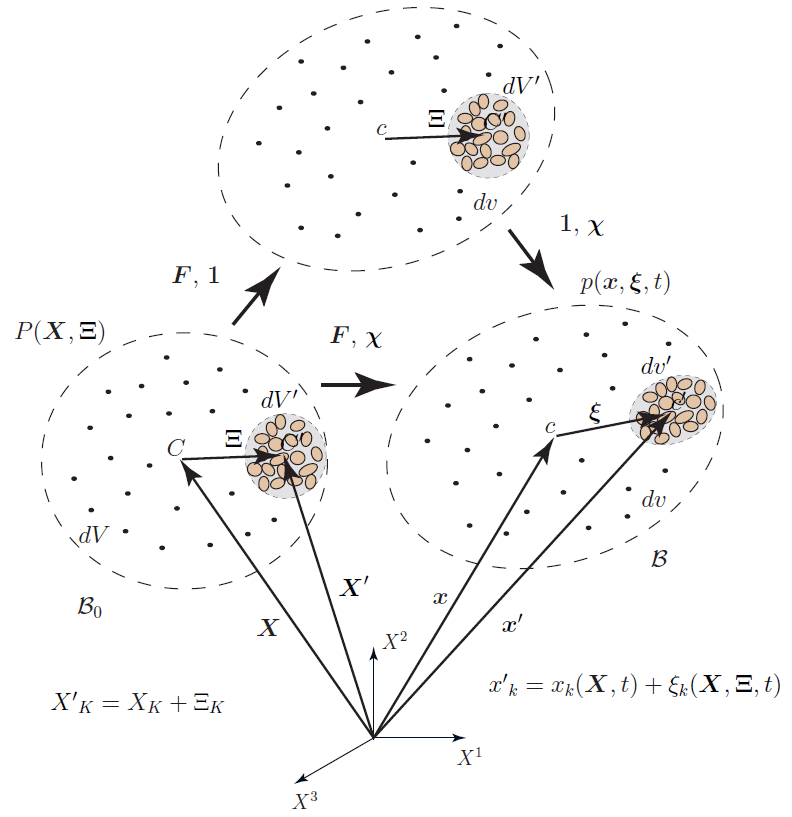
\includegraphics[width=0.9\textwidth]{micromorphic.png}
\end{figure}
\end{column}
\end{columns}
\end{frame}

\begin{frame}{Kinematics}
\begin{align*}
\VEC{X}' &= \VEC{X}+\VEC{\Xi}\\
\VEC{x}' &= \VEC{x}+\VEC{\xi}\\
\end{align*}

We assume that $\LTN{\Xi_{I}} << 1$ and that a linear mapping $\TEN{\Xi}$ exists such that

\begin{align*}
\xi_i &= \chi_{iI} \Xi_I
\end{align*}

The deformation gradient $\TEN{F}$ is defined such that
\begin{align*}
F_{iI} &= \frac{\partial x_i}{\partial X_I}\\
\end{align*}
\end{frame}

\begin{frame}{Definitions of Macro-scale quantities}

We make the following definitions of the macro scale quantities

\begin{equation}
\begin{aligned}[c]
\rho dv &\defeq \int_{dv} \rho' dv'\\
\rho i_{ij} dv &\defeq \int_{dv} \rho' \xi_i \xi_j dv'\\
\sigma_{ij} n_i da &\defeq \int_{da} \sigma_{ij}' n_i' da'\\
\rho f_j dv &\defeq \int_{dv} \rho' f_j' dv'\\
\rho a_j dv &\defeq \int_{dv} \rho' a_j' dv'\\
\end{aligned}
\begin{aligned}
s_{ij} dv &\defeq \int_{dv} \sigma_{ij} dv'\\
m_{ijk} n_i da &\defeq \int_{da} \sigma_{ij}' \xi_k n_i da'\\
\rho l_{jk} dv &\defeq \int_{dv} \rho' \xi_k f_j' dv'\\
\rho \omega_{jk} dv &\defeq \int_{dv} \rho' \xi_k \ddot{\xi}_j dv'\\
\end{aligned}
\end{equation}

\end{frame}

\begin{frame}{Balance Equations}

\begin{itemize}
\item {Balance of Mass 
\begin{equation}
\frac{D \rho}{Dt} + \frac{\partial v_i}{\partial x_i} = 0\
\end{equation}
}
\item{Balance of Linear Momentum
\begin{equation}
\sigma_{ij,i} + \rho\left(f_j - a_j\right) = 0
\end{equation}
}
\item{Balance of First Moment of Momentum
\begin{equation}
\sigma_{kj} + m_{ijk,i} - s_{kj} + \rho\left(l_{jk} - \omega_{jk}\right) = 0
\end{equation}
}

We leave out the balance of energy and the entropy inequality for brevity.
\end{itemize}

\end{frame}

\begin{frame}{The Finite Element Form}

We can write the weak form of the balance of linear momentum as
\begin{align*}
\int_{\partial \mathcal{B}} w_j \sigma_{ij} n_i da +\int_{\mathcal{B}} w_j \rho f_j dv - \int_{\mathcal{B}}w_{j,i} \sigma_{ij} - \int_{\mathcal{B}} w_j \rho a_j  dv &= 0\\
\end{align*}

where $w_j$ is the weighting function.

\end{frame}

\begin{frame}{The Finite Element Form}

Similarly,

\begin{align*}
\int_{\mathcal{B}} \left\{\eta_{ij} \left(\sigma_{ij} - s_{ij}\right) - \eta_{ij,k} m_{kji} \right\}dv + \int_{\partial \mathcal{B}} \eta_{ij} m_{ji}  da + \int_{\mathcal{B}} \rho \eta_{ij} l_{ji}dv&\\
- \int_{\mathcal{B}} \rho \eta_{ij} \omega_{ji} dv&= 0\\
\end{align*}


To continue, we define
\begin{align*}
w_j = \sum_n N^n(x) c_{j}^n\ \ \ \
\eta_{ij} = \sum_n N^n(x) \eta_{ij}^n\\
\end{align*}

\end{frame}

\begin{frame}{The Finite Element Form}

Which means
\begin{align*}
\sum_{n} c_j^n \bigg\{\int_{\partial \mathcal{B}} N^n \sigma_{ij} n_i da +\int_{\mathcal{B}} N^n \rho f_j dv &\\- \int_{\mathcal{B}}N_{,i}^N \sigma_{ij}
- \int_{\mathcal{B}} N^n \rho a_j  dv\bigg\} &= 0\\
\sum_{n} \eta_{ij} \bigg\{\int_{\mathcal{B}} \left\{N^n \left(\sigma_{ij} - s_{ij}\right) - N_{,k}^n m_{kji} \right\}dv\\
+ \int_{\partial \mathcal{B}} N^n m_{ji}  da + \int_{\mathcal{B}} \rho N^n l_{ji}dv - \int_{\mathcal{B}} \rho N^n \omega_{ji} dv\bigg\}&= 0\\
\end{align*}

\end{frame}

\begin{frame}{The Finite Element Form}

We now define the forces on the nodes as
\begin{align*}
F_{j}^{n,int} &\defeq \int_{\mathcal{B}}N_{,i}^N \sigma_{ij}\\
F_{j}^{n,ext} &\defeq \int_{\partial \mathcal{B}} N^n \sigma_{ij} n_i da +\int_{\mathcal{B}} N^n \rho f_j dv\\
F_{j}^{n,kin} &\defeq \int_{\mathcal{B}} N^n \rho a_j  dv\\
\Rightarrow\ \sum_{n} c_j^n &\left\{F_{j}^{n,ext} - F_{j}^{n,int} - F_{j}^{n,kin} \right\} = 0\\
\end{align*}

\end{frame}

\begin{frame}{The Finite Element Form}

The moments on the nodes are
\begin{align*}
M_{ij}^{n,int} &\defeq \int_{\mathcal{B}} \left\{N_{,k}^n m_{kji} + N^n \left(s_{ij} - \sigma_{ij}\right)\right\}dv\\
M_{ij}^{n,ext} &\defeq \int_{\partial \mathcal{B}} N^n m_{ji}  da + \int_{\mathcal{B}} \rho N^n l_{ji}dv\\
M_{ij}^{n,kin} &\defeq \int_{\mathcal{B}} \rho N^n \omega_{ji} dv\\
\Rightarrow\ \sum_{n} \eta_{ij}^n &\left\{M_{ij}^{n,ext} - M_{ij}^{n,int} - M_{ij}^{n,kin} \right\} = 0\\
\end{align*}

which is a similar form to the balance of linear momentum.

\end{frame}

\begin{frame}{The Finite Element Form}

Because $c_j$ and $\eta_{ij}$ are arbitrary (except where the dirichlet boundary conditions are applied and they are zero) we can write
\begin{align*}
F_{j}^{n,ext} - F_{j}^{n,int} - F_{j}^{n,kin} &= 0_j\\
M_{ij}^{n,ext} - M_{ij}^{n,int} - M_{ij}^{n,kin} &= 0_{ij}
\end{align*}

Which is in a root finding form for Newton-Raphson iteration.

\begin{equation}
\begin{aligned}
F_{j}^{n,ext} - F_{j}^{n,int} - F_{j}^{n,kin} &= \mathcal{F}_j^n\\
M_{ij}^{n,ext} - M_{ij}^{n,int} - M_{ij}^{n,kin} &= \mathcal{M}_{ij}^n
\end{aligned}
\label{eqn:residual_form}
\end{equation}


\end{frame}

\begin{frame}{Newton-Raphson Solution}

We combine the forces and moments into a single residual (details in Theory Manual) and write

\begin{equation}
\begin{aligned}
\mathcal{R}_i &= \left[\begin{array}{c}
\mathcal{F}_k^1\\
\mathcal{M}_{kl}^1\\
\mathcal{F}_k^2\\
\mathcal{M}_{kl}^2\\
\vdots\\
\end{array}\right]_i^{ext}
\end{aligned}
\end{equation}

\end{frame}

%\begin{frame}{Newton-Raphson Solution}
%We compute the derivative of Equation~\ref{eqn:residual_form} with respect to the degree of freedom vector $U_l$ to find
%
%\begin{align*}
%\frac{\partial \mathcal{F}_j^n}{\partial U_l} &= \frac{F_{j}^{n,ext}}{\partial U_l} - \frac{F_{j}^{n,int}}{\partial U_l} - \frac{F_{j}^{n,kin}}{\partial U_l}\\
%\frac{\partial \mathcal{M}_{ij}^n}{\partial U_l} &= \frac{M_{ij}^{n,ext}}{\partial U_l} - \frac{M_{ij}^{n,int}}{\partial U_l} - \frac{M_{ij}^{n,kin}}{\partial U_l}
%\end{align*}
%
%which means
%\begin{align*}
%&= \mathcal{R}_i^k + 
%\end{align*}
%
%\end{frame}

\begin{frame}{Newton-Raphson Solution}

We desire the residual at the next iteration to be zero so we write
\begin{equation}
\begin{aligned}
0 &= R_i^k + \frac{\partial R_i}{\partial U_j} \Delta U_j\\
\Rightarrow\ -\frac{\partial R_i}{\partial U_j} \Delta U_j &= R_i^k\\
\end{aligned}
\end{equation}

We now introduce
\begin{align*}
\Delta U_j &= \Delta t \dot{U}_j\\
\dot{U}_j &= \alpha \dot{U}_j^{k+1} + \left(1-\alpha\right) \dot{U}_j^{k}
\end{align*}

where $\alpha = 0$ indicates an explicit method and $\alpha = 1$ indicates an implicit method.

\end{frame}

\begin{frame}{Newton-Raphson Solution}

We now rewrite the solution to find
\begin{equation}
\begin{aligned}
-\frac{\partial R_i}{\partial U_j} \Delta t \left(\alpha \dot{U}_j^{k+1} + \left(1-\alpha\right) \dot{U}_j^{k}\right) &= R_i^k\\
\Rightarrow\ -\frac{\partial R_i}{\partial U_j} \Delta t \alpha \dot{U}_j^{k+1} &= R_i^k + \left(1-\alpha\right) \Delta t \frac{\partial R_i}{\partial U_j} \dot{U}_j^k\\
\Rightarrow\ - \frac{\partial R_i}{\partial U_j} \Delta U_j^{k+1} &= \frac{1}{\alpha} \left[R_i^k + \left(1-\alpha\right) \frac{\partial R_i}{\partial U_j} \Delta U_j^k\right]\\
\end{aligned}
\end{equation}

\end{frame}

\begin{frame}{Solution Strategy}

The coupled PDEs will be solved using a total lagrangian finite element strategy. In other words, we will map back to the reference configuration and solve the equations of motion there. See the theory manual for additional details.

\end{frame}

\begin{frame}{Software Environment}

\begin{columns}
\begin{column}{0.5\textwidth}
\begin{itemize}
\item {The code will be developed in Python
\begin{itemize}
\item Rapid iteration
\item Matrix solvers available
\item Integrated testing environment (unittest)
\end{itemize}
}
\item{The code will be divided into four major modules
\begin{itemize}
\item fea\_driver.py
\item micro\_element.py
\item hex8.py
\item constitutive model
\end{itemize}
}
\end{itemize}
\end{column}
\begin{column}{0.5\textwidth}
\begin{itemize}
\item{
Testing will be broken into two components
\begin{itemize}
\item Unit tests
\item Regression tests
\end{itemize}
}
\item{
Version control will be handled with Git
}
\end{itemize}
\end{column}
\end{columns}

\end{frame}

\begin{frame}{Documentation Plan}

\begin{columns}
\begin{column}{0.5\textwidth}
\begin{itemize}
\item{All attempts will be made to follow Python style guides when possible
\begin{itemize}
\item{Functions should be named as what they actively achieve}
\item{Variable names should be unambiguous as to their contents}
\item{All functions should have a documentation string}
\end{itemize}
}
\end{itemize}
\end{column}
\begin{column}{0.5\textwidth}
\begin{itemize}
\item{
The programmers manual will illuminate the primary routines of the code and what will be required to develop new constitutive models.
}
\item{The theory manual will clearly describe all derivations used in the code}
\end{itemize}
\end{column}
\end{columns}

\end{frame}

\begin{frame}{Cost Estimates}

Note: Completed does not mean totally debugged!

\begin{table}[htb!]
\centering
\begin{tabular}{|c|c|c|}
\hline
Task & Dates & Status\\
\hline
\hline
Derive equations of motion & May 01 - June 11 & \cellcolor{green!25}Completed\\
\hline
Implementation strategy & June 11 - June 18 & \cellcolor{green!25}Completed\\
\hline
Development of & June 11 - August 11 & \cellcolor{green!25} Completed \\
utility routines & & \cellcolor{green!25}\\
\hline
Implementation of &  June 20 - August 01 & \cellcolor{green!25} Completed\\
residuals and tangents & &\cellcolor{green!25}\\
\hline
Finite Element Driver & August 2 - August 5 & \cellcolor{yellow!25} On Schedule\\
\hline
Manufactured Solutions & August 6 - August 10 & \cellcolor{green!25} Completed\\
\hline
Documentation/Report & August 6 - August 10 & \cellcolor{yellow!25} On schedule\\
\hline
\end{tabular}
\label{table:development_status}
\end{table}

\end{frame}





\end{document}